% Options for packages loaded elsewhere
\PassOptionsToPackage{unicode}{hyperref}
\PassOptionsToPackage{hyphens}{url}
\PassOptionsToPackage{dvipsnames,svgnames,x11names}{xcolor}
%
\documentclass[
  letterpaper,
  DIV=11,
  numbers=noendperiod]{scrartcl}

\usepackage{amsmath,amssymb}
\usepackage{lmodern}
\usepackage{iftex}
\ifPDFTeX
  \usepackage[T1]{fontenc}
  \usepackage[utf8]{inputenc}
  \usepackage{textcomp} % provide euro and other symbols
\else % if luatex or xetex
  \usepackage{unicode-math}
  \defaultfontfeatures{Scale=MatchLowercase}
  \defaultfontfeatures[\rmfamily]{Ligatures=TeX,Scale=1}
\fi
% Use upquote if available, for straight quotes in verbatim environments
\IfFileExists{upquote.sty}{\usepackage{upquote}}{}
\IfFileExists{microtype.sty}{% use microtype if available
  \usepackage[]{microtype}
  \UseMicrotypeSet[protrusion]{basicmath} % disable protrusion for tt fonts
}{}
\makeatletter
\@ifundefined{KOMAClassName}{% if non-KOMA class
  \IfFileExists{parskip.sty}{%
    \usepackage{parskip}
  }{% else
    \setlength{\parindent}{0pt}
    \setlength{\parskip}{6pt plus 2pt minus 1pt}}
}{% if KOMA class
  \KOMAoptions{parskip=half}}
\makeatother
\usepackage{xcolor}
\setlength{\emergencystretch}{3em} % prevent overfull lines
\setcounter{secnumdepth}{-\maxdimen} % remove section numbering
% Make \paragraph and \subparagraph free-standing
\ifx\paragraph\undefined\else
  \let\oldparagraph\paragraph
  \renewcommand{\paragraph}[1]{\oldparagraph{#1}\mbox{}}
\fi
\ifx\subparagraph\undefined\else
  \let\oldsubparagraph\subparagraph
  \renewcommand{\subparagraph}[1]{\oldsubparagraph{#1}\mbox{}}
\fi


\providecommand{\tightlist}{%
  \setlength{\itemsep}{0pt}\setlength{\parskip}{0pt}}\usepackage{longtable,booktabs,array}
\usepackage{calc} % for calculating minipage widths
% Correct order of tables after \paragraph or \subparagraph
\usepackage{etoolbox}
\makeatletter
\patchcmd\longtable{\par}{\if@noskipsec\mbox{}\fi\par}{}{}
\makeatother
% Allow footnotes in longtable head/foot
\IfFileExists{footnotehyper.sty}{\usepackage{footnotehyper}}{\usepackage{footnote}}
\makesavenoteenv{longtable}
\usepackage{graphicx}
\makeatletter
\def\maxwidth{\ifdim\Gin@nat@width>\linewidth\linewidth\else\Gin@nat@width\fi}
\def\maxheight{\ifdim\Gin@nat@height>\textheight\textheight\else\Gin@nat@height\fi}
\makeatother
% Scale images if necessary, so that they will not overflow the page
% margins by default, and it is still possible to overwrite the defaults
% using explicit options in \includegraphics[width, height, ...]{}
\setkeys{Gin}{width=\maxwidth,height=\maxheight,keepaspectratio}
% Set default figure placement to htbp
\makeatletter
\def\fps@figure{htbp}
\makeatother

\KOMAoption{captions}{tableheading}
\makeatletter
\makeatother
\makeatletter
\makeatother
\makeatletter
\@ifpackageloaded{caption}{}{\usepackage{caption}}
\AtBeginDocument{%
\ifdefined\contentsname
  \renewcommand*\contentsname{Table of contents}
\else
  \newcommand\contentsname{Table of contents}
\fi
\ifdefined\listfigurename
  \renewcommand*\listfigurename{List of Figures}
\else
  \newcommand\listfigurename{List of Figures}
\fi
\ifdefined\listtablename
  \renewcommand*\listtablename{List of Tables}
\else
  \newcommand\listtablename{List of Tables}
\fi
\ifdefined\figurename
  \renewcommand*\figurename{Figure}
\else
  \newcommand\figurename{Figure}
\fi
\ifdefined\tablename
  \renewcommand*\tablename{Table}
\else
  \newcommand\tablename{Table}
\fi
}
\@ifpackageloaded{float}{}{\usepackage{float}}
\floatstyle{ruled}
\@ifundefined{c@chapter}{\newfloat{codelisting}{h}{lop}}{\newfloat{codelisting}{h}{lop}[chapter]}
\floatname{codelisting}{Listing}
\newcommand*\listoflistings{\listof{codelisting}{List of Listings}}
\makeatother
\makeatletter
\@ifpackageloaded{caption}{}{\usepackage{caption}}
\@ifpackageloaded{subcaption}{}{\usepackage{subcaption}}
\makeatother
\makeatletter
\@ifpackageloaded{tcolorbox}{}{\usepackage[many]{tcolorbox}}
\makeatother
\makeatletter
\@ifundefined{shadecolor}{\definecolor{shadecolor}{rgb}{.97, .97, .97}}
\makeatother
\makeatletter
\makeatother
\ifLuaTeX
  \usepackage{selnolig}  % disable illegal ligatures
\fi
\IfFileExists{bookmark.sty}{\usepackage{bookmark}}{\usepackage{hyperref}}
\IfFileExists{xurl.sty}{\usepackage{xurl}}{} % add URL line breaks if available
\urlstyle{same} % disable monospaced font for URLs
\hypersetup{
  pdftitle={Report 2021/2022},
  colorlinks=true,
  linkcolor={blue},
  filecolor={Maroon},
  citecolor={Blue},
  urlcolor={Blue},
  pdfcreator={LaTeX via pandoc}}

\title{Report 2021/2022}
\author{}
\date{}

\begin{document}
\maketitle
\ifdefined\Shaded\renewenvironment{Shaded}{\begin{tcolorbox}[borderline west={3pt}{0pt}{shadecolor}, boxrule=0pt, sharp corners, frame hidden, breakable, interior hidden, enhanced]}{\end{tcolorbox}}\fi

\renewcommand*\contentsname{Table of contents}
{
\hypersetup{linkcolor=}
\setcounter{tocdepth}{2}
\tableofcontents
}
\hypertarget{acknowledgements}{%
\subsection{Acknowledgements}\label{acknowledgements}}

Friends, Romans, countrymen, lend me your ears; I come to bury Caesar,
not to praise him. The evil that men do lives after them; The good is
oft interred with their bones; So let it be with Caesar. The noble
Brutus Hath told you Caesar was ambitious: If it were so, it was a
grievous fault, And grievously hath Caesar answer'd it. Here, under
leave of Brutus and the rest-- For Brutus is an honourable man; So are
they all, all honourable men-- Come I to speak in Caesar's funeral. He
was my friend, faithful and just to me: But Brutus says he was
ambitious; And Brutus is an honourable man. He hath brought many
captives home to Rome Whose ransoms did the general coffers fill: Did
this in Caesar seem ambitious?

\hypertarget{executive-summary}{%
\subsection{Executive Summary}\label{executive-summary}}

Friends, Romans, countrymen, lend me your ears; I come to bury Caesar,
not to praise him. The evil that men do lives after them; The good is
oft interred with their bones; So let it be with Caesar. The noble
Brutus Hath told you Caesar was ambitious: If it were so, it was a
grievous fault, And grievously hath Caesar answer'd it. Here, under
leave of Brutus and the rest-- For Brutus is an honourable man; So are
they all, all honourable men-- Come I to speak in Caesar's funeral. He
was my friend, faithful and just to me: But Brutus says he was
ambitious; And Brutus is an honourable man. He hath brought many
captives home to Rome Whose ransoms did the general coffers fill: Did
this in Caesar seem ambitious?

\hypertarget{background}{%
\subsection{Background}\label{background}}

Friends, Romans, countrymen, lend me your ears; I come to bury Caesar,
not to praise him. The evil that men do lives after them; The good is
oft interred with their bones; So let it be with Caesar. The noble
Brutus Hath told you Caesar was ambitious: If it were so, it was a
grievous fault, And grievously hath Caesar answer'd it. Here, under
leave of Brutus and the rest-- For Brutus is an honourable man; So are
they all, all honourable men-- Come I to speak in Caesar's funeral. He
was my friend, faithful and just to me: But Brutus says he was
ambitious; And Brutus is an honourable man. He hath brought many
captives home to Rome Whose ransoms did the general coffers fill: Did
this in Caesar seem ambitious?\#\# Aim

\hypertarget{methodology}{%
\subsection{Methodology}\label{methodology}}

Quant: Compare results from all schools -- 2021 and 2022

Demographics of schools participating in the self-assessment tool (SAT):
2021 \& 2022

Pie charts side-by-side: 2021 and 2022. Sector, Type, SES, ADII,
Metro/non-metro; 2022 only: Engagement A (Low, High) and Engagement B
(Low, Medium, High)

\begin{figure}

\begin{minipage}[t]{0.50\linewidth}

{\centering 

}

\end{minipage}%
%
\begin{minipage}[t]{0.50\linewidth}

{\centering 

Plot 1

}

\end{minipage}%
\newline
\begin{minipage}[t]{0.50\linewidth}

{\centering 

}

\end{minipage}%
%
\begin{minipage}[t]{0.50\linewidth}

{\centering 

Plot 2

}

\end{minipage}%
\newline
\begin{minipage}[t]{0.50\linewidth}

{\centering 

Participants by sector

}

\end{minipage}%

\end{figure}

Figure 3. Participants by SES

Participants by SES

Participants by SES

Figure 4. Participants by ADII

Participants by ADII

Participants by ADII

Figure 5. Participants by location: metro / non-metro

Participants by location: metro / non-metro

Participants by location: metro / non-metro

Figure 6. Participants by DET region N/A Figure 7. Participants by
eSmart status N/A

Figure 8. Part A: average (median) number of eSmart action items
completed by sector (out of 23)

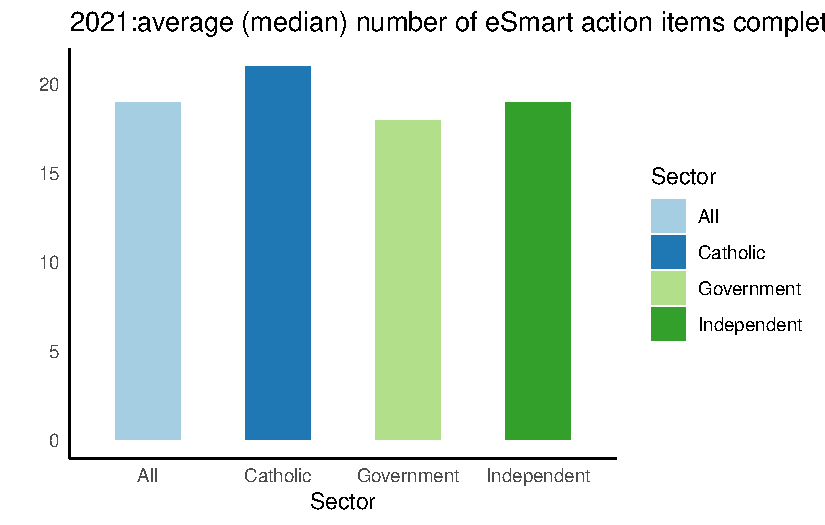
\includegraphics{report_files/figure-pdf/unnamed-chunk-8-1.pdf}

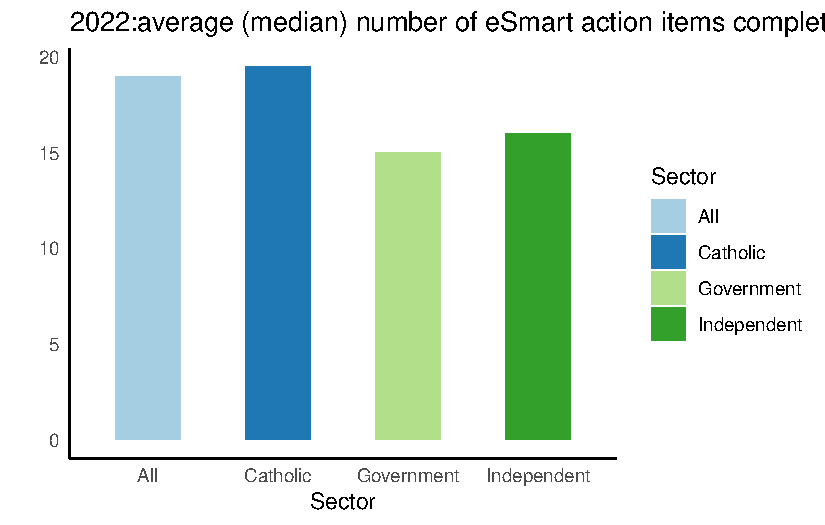
\includegraphics{report_files/figure-pdf/unnamed-chunk-8-2.pdf}

Figure 9. Part A: number of eSmart action items achieved (out of 23) by
sector

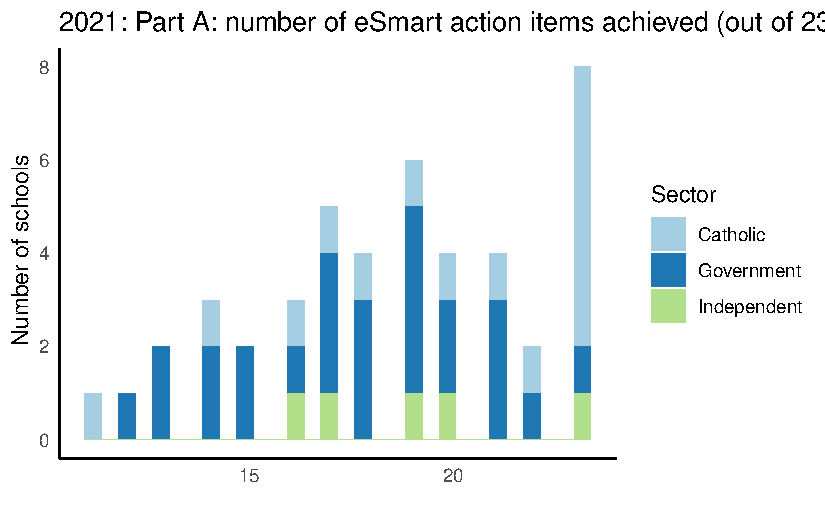
\includegraphics{report_files/figure-pdf/unnamed-chunk-9-1.pdf}

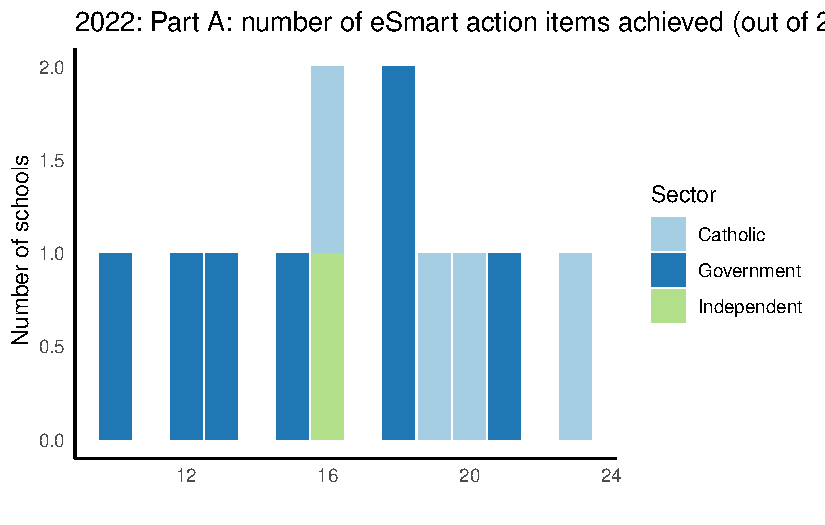
\includegraphics{report_files/figure-pdf/unnamed-chunk-9-2.pdf}

Figure 10. Part A: average (mean) completion of eSmart action items -
all schools by Domain

\begin{verbatim}
# A tibble: 2 x 10
  `DOMAIN: DATA` DOMAI~1 DOMAI~2 DOMAI~3 DOMAI~4 PRE-S~5 PRE-S~6 POST-~7 POST-~8
           <dbl>   <dbl>   <dbl>   <dbl>   <dbl>   <dbl>   <dbl>   <dbl>   <dbl>
1             51      45      40      54      63       5       5       6       6
2             33      45      43      51      60       7       7       7       7
# ... with 1 more variable: `TOTAL: Domains` <dbl>, and abbreviated variable
#   names 1: `DOMAIN: GATEWAY BEHAVIOURS`, 2: `DOMAIN: REPORTING`,
#   3: `DOMAIN: RESPONSE`, 4: `DOMAIN: SCHOOL CLIMATE`, 5: `PRE-SURVEY1`,
#   6: `PRE-SURVEY2`, 7: `POST-SURVEY1`, 8: `POST-SURVEY2`
# i Use `colnames()` to see all variable names
\end{verbatim}

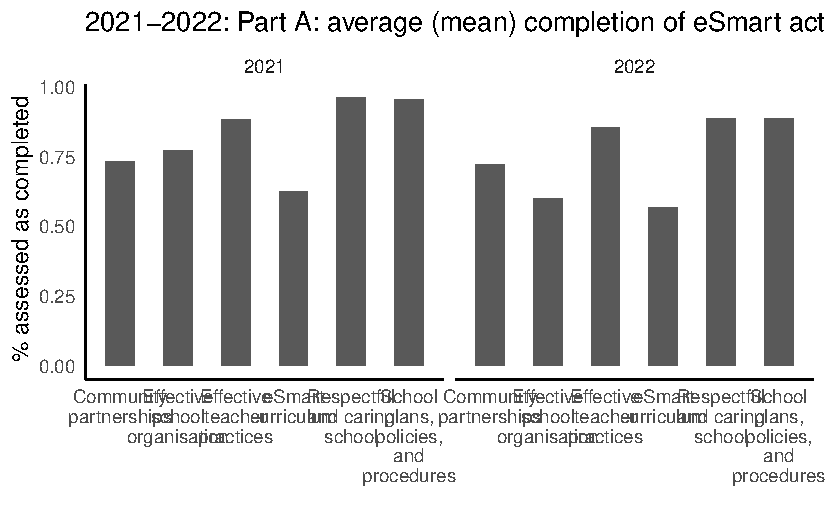
\includegraphics{report_files/figure-pdf/unnamed-chunk-12-1.pdf}

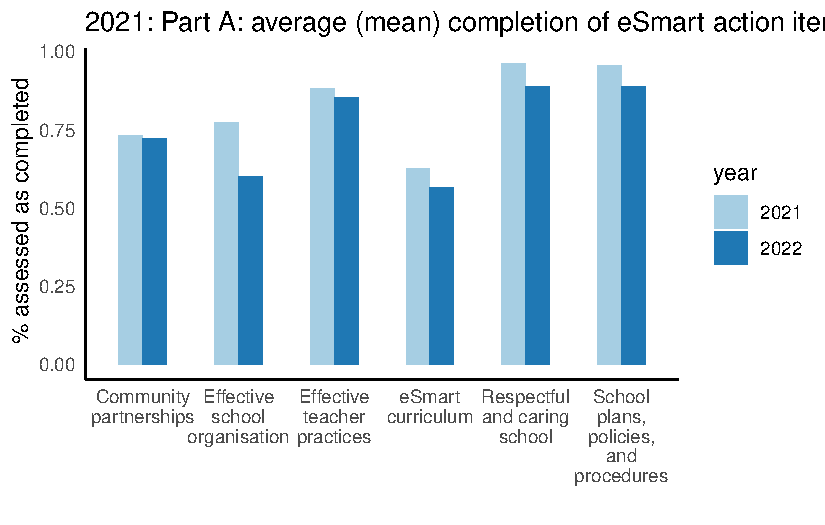
\includegraphics{report_files/figure-pdf/unnamed-chunk-12-2.pdf}

Figure 11. Part A: average (mean) completion of eSmart action items by
Domain by sector

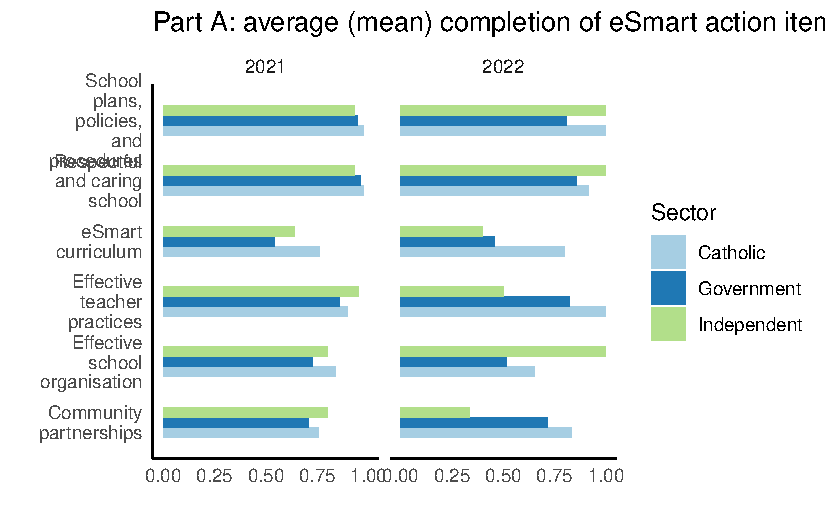
\includegraphics{report_files/figure-pdf/unnamed-chunk-13-1.pdf}

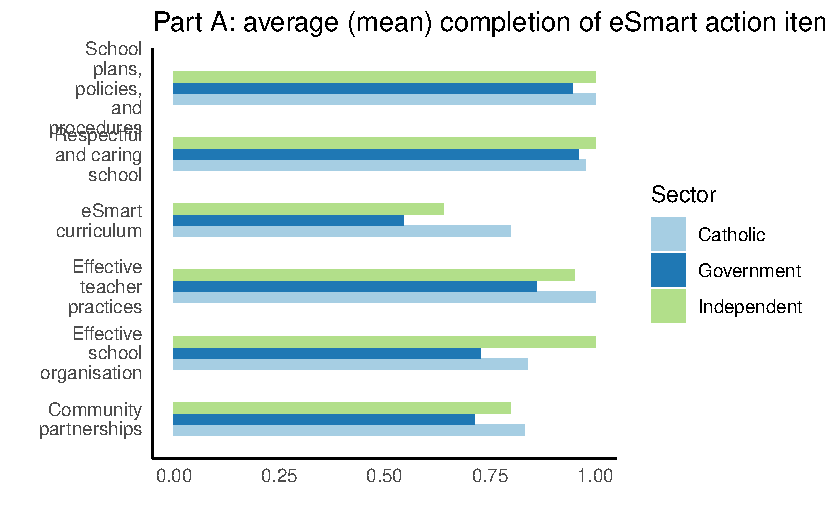
\includegraphics{report_files/figure-pdf/unnamed-chunk-13-2.pdf}

Figure 12. Part A: Average (mean) completion by Domain by SES.

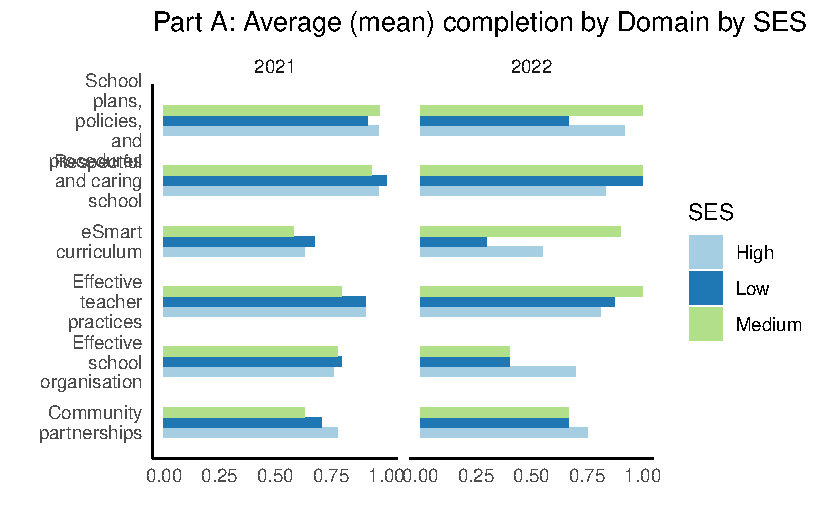
\includegraphics{report_files/figure-pdf/unnamed-chunk-14-1.pdf}

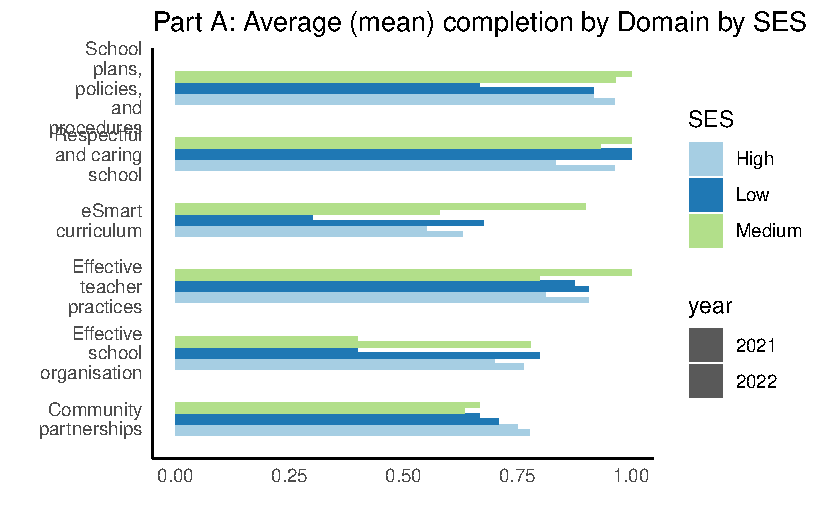
\includegraphics{report_files/figure-pdf/unnamed-chunk-14-2.pdf}

Figure 13. Part B: results by Focus Area - all schools

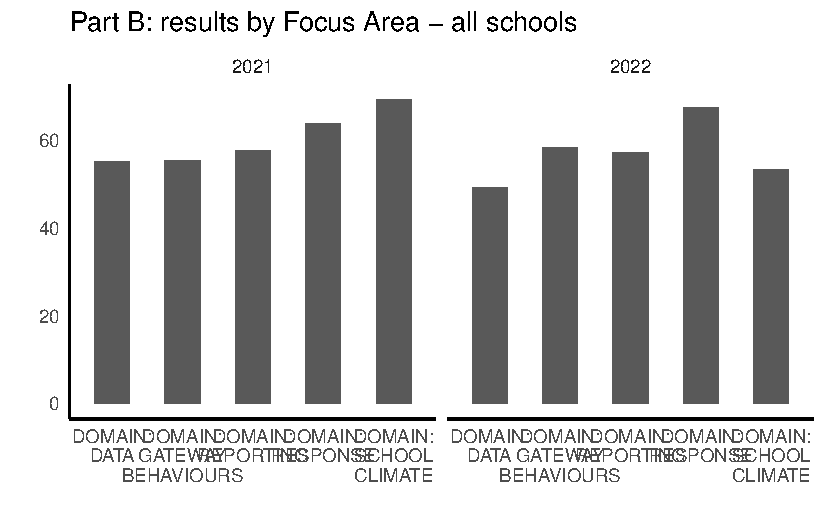
\includegraphics{report_files/figure-pdf/unnamed-chunk-15-1.pdf}

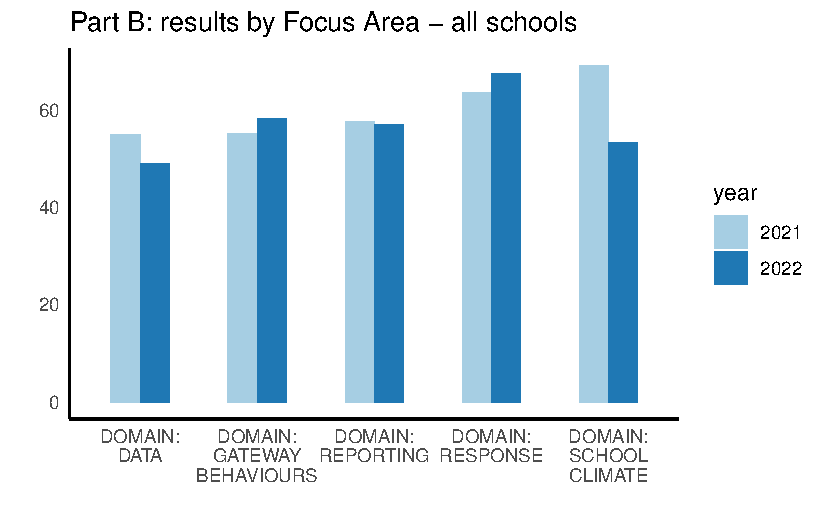
\includegraphics{report_files/figure-pdf/unnamed-chunk-15-2.pdf}

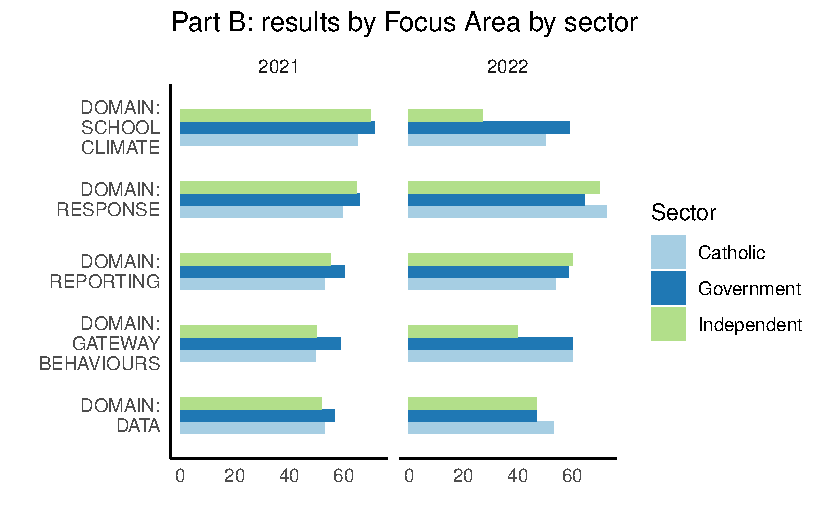
\includegraphics{report_files/figure-pdf/unnamed-chunk-16-1.pdf}

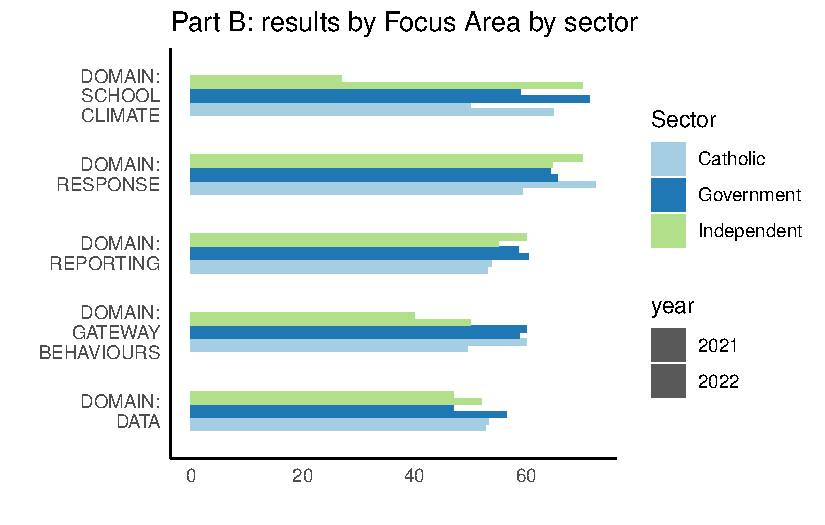
\includegraphics{report_files/figure-pdf/unnamed-chunk-16-2.pdf}

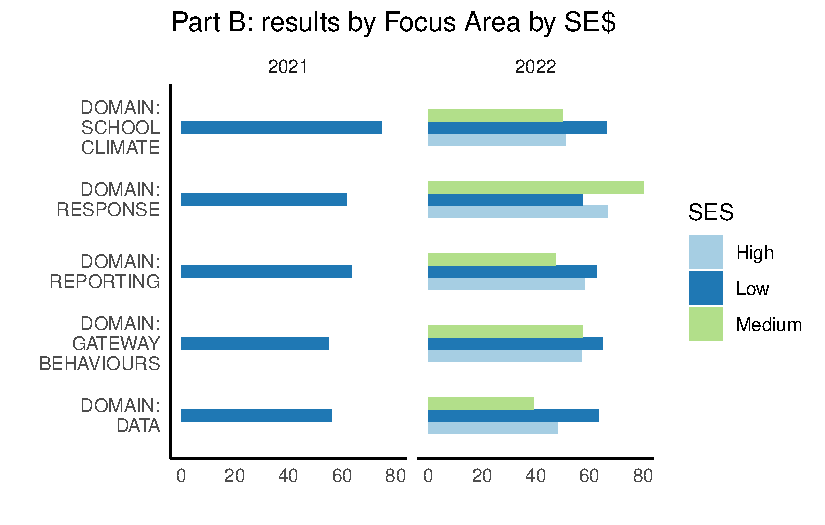
\includegraphics{report_files/figure-pdf/unnamed-chunk-17-1.pdf}

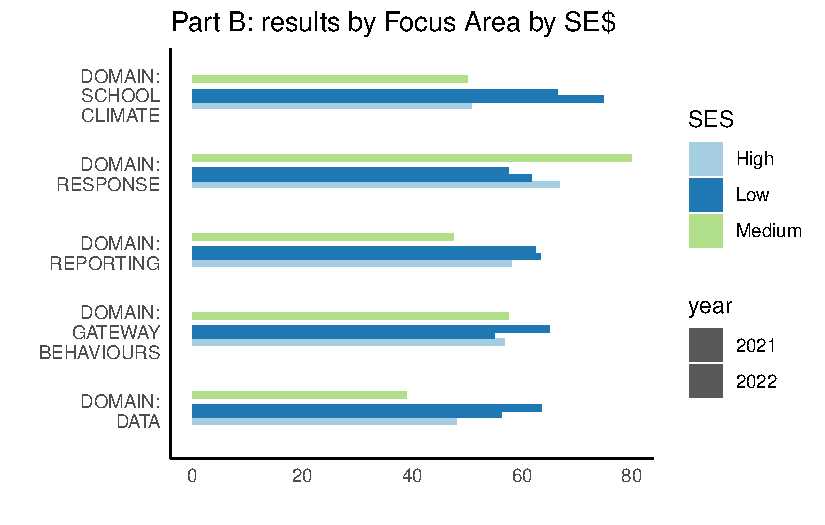
\includegraphics{report_files/figure-pdf/unnamed-chunk-17-2.pdf}

Figure 16. Part B: results by Focus Area by school type

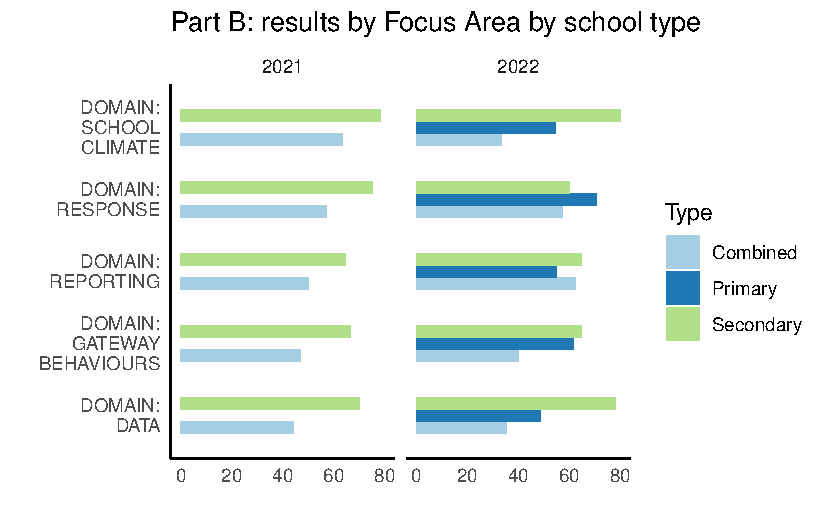
\includegraphics{report_files/figure-pdf/unnamed-chunk-18-1.pdf}

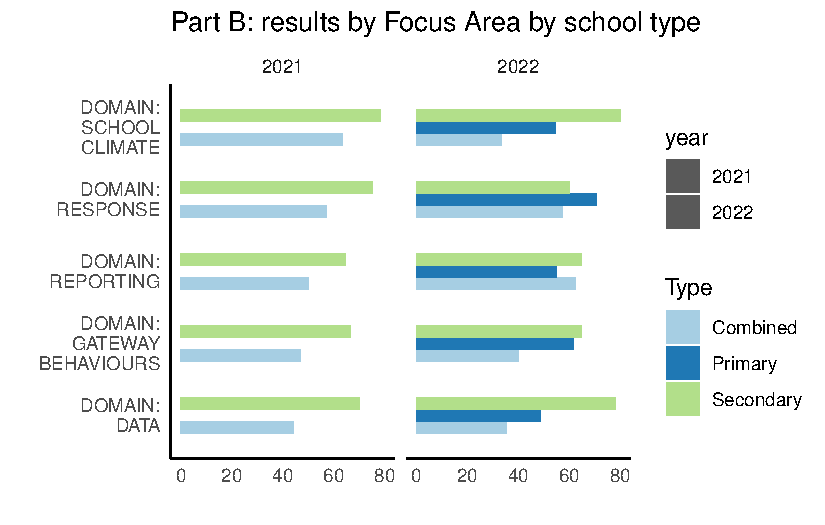
\includegraphics{report_files/figure-pdf/unnamed-chunk-18-2.pdf}

Figure 17. Part B: progress in eSmart journey - all schools - no data

Engagement - 2022 data only

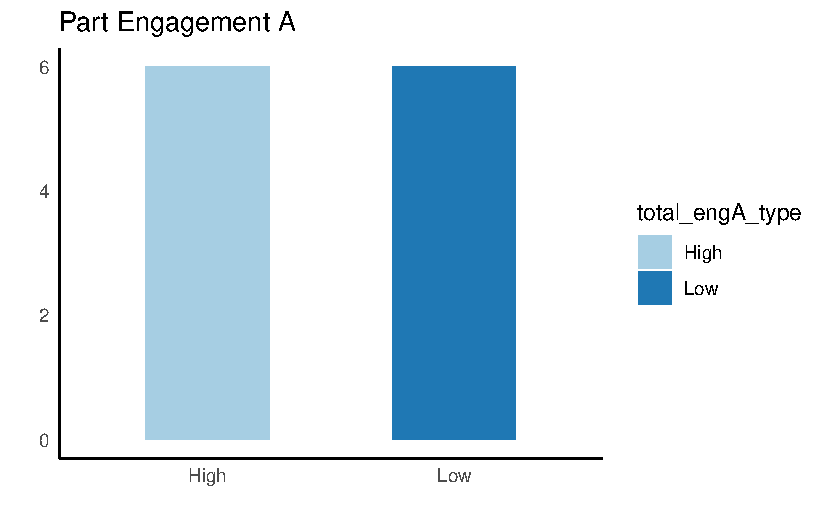
\includegraphics{report_files/figure-pdf/unnamed-chunk-19-1.pdf}

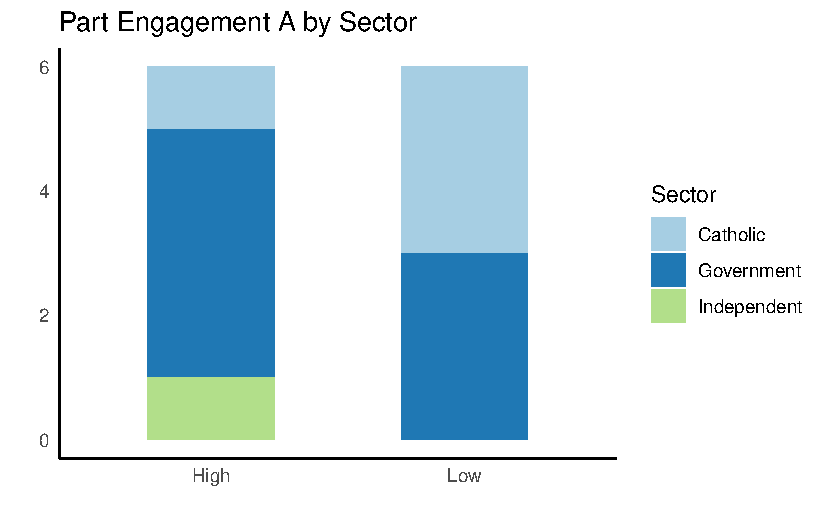
\includegraphics{report_files/figure-pdf/unnamed-chunk-19-2.pdf}

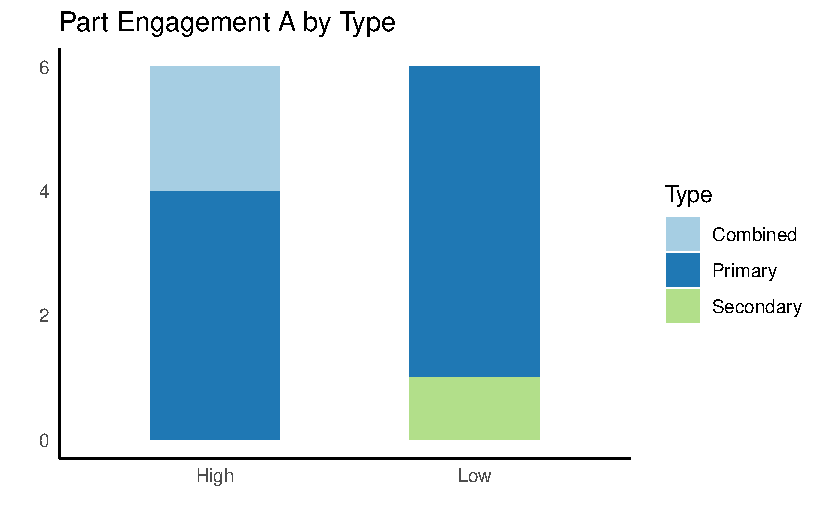
\includegraphics{report_files/figure-pdf/unnamed-chunk-19-3.pdf}

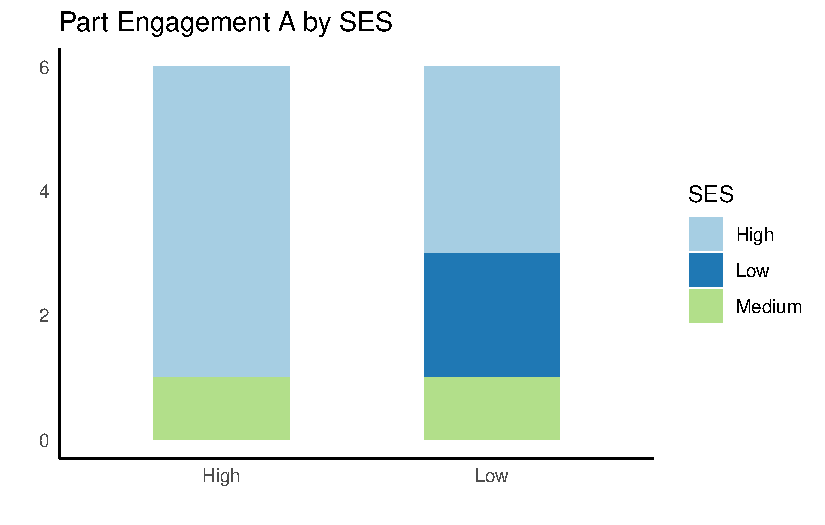
\includegraphics{report_files/figure-pdf/unnamed-chunk-19-4.pdf}

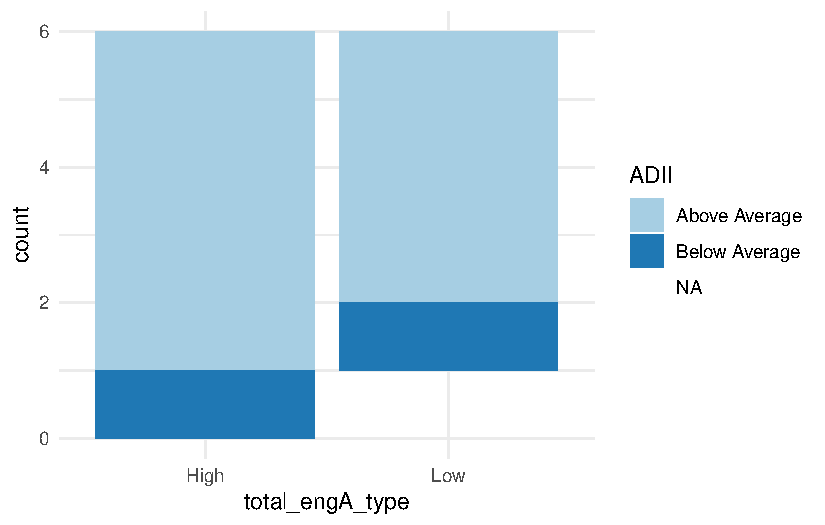
\includegraphics{report_files/figure-pdf/unnamed-chunk-19-5.pdf}

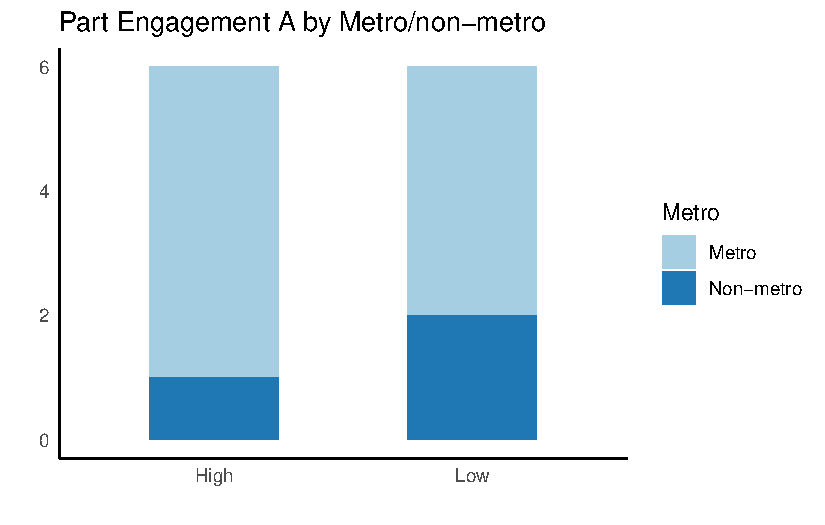
\includegraphics{report_files/figure-pdf/unnamed-chunk-19-6.pdf}

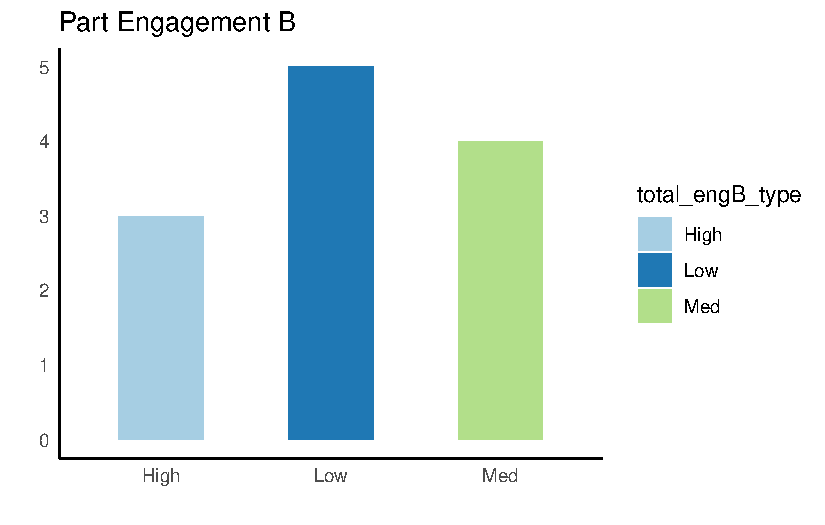
\includegraphics{report_files/figure-pdf/unnamed-chunk-19-7.pdf}

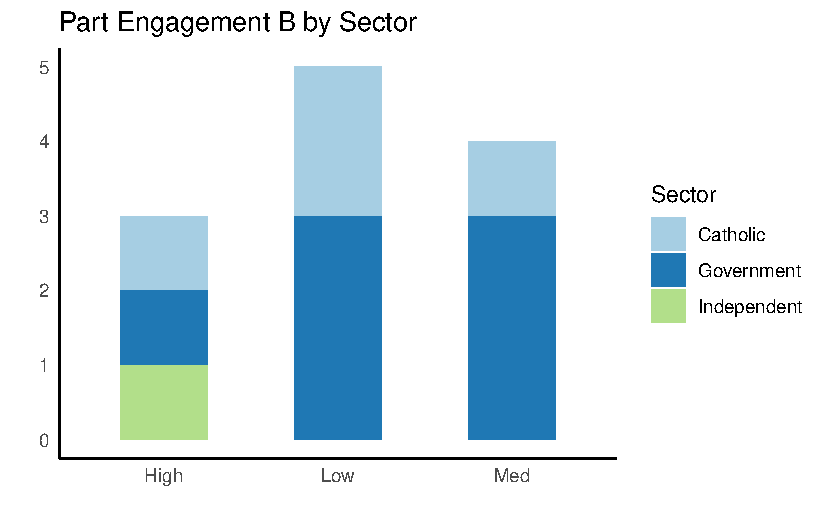
\includegraphics{report_files/figure-pdf/unnamed-chunk-19-8.pdf}

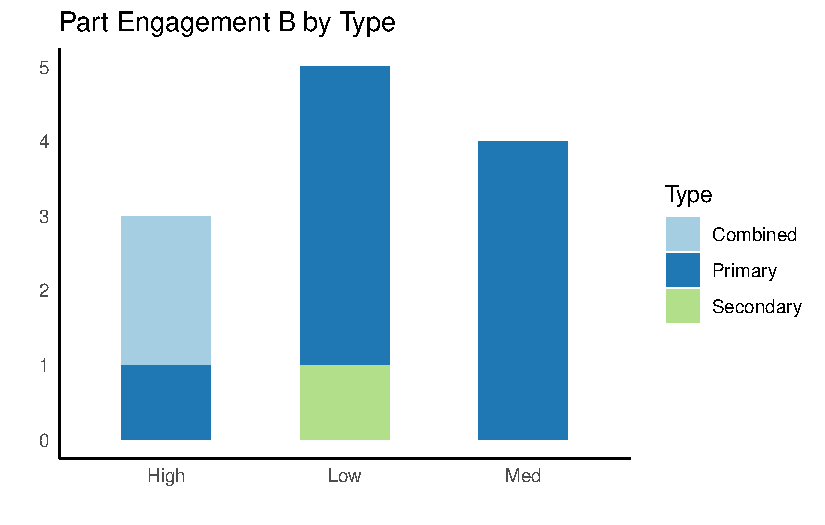
\includegraphics{report_files/figure-pdf/unnamed-chunk-19-9.pdf}

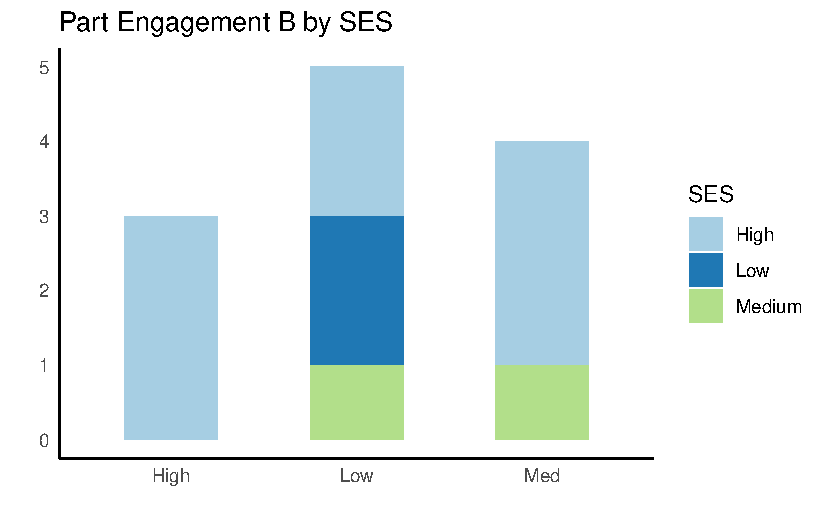
\includegraphics{report_files/figure-pdf/unnamed-chunk-19-10.pdf}

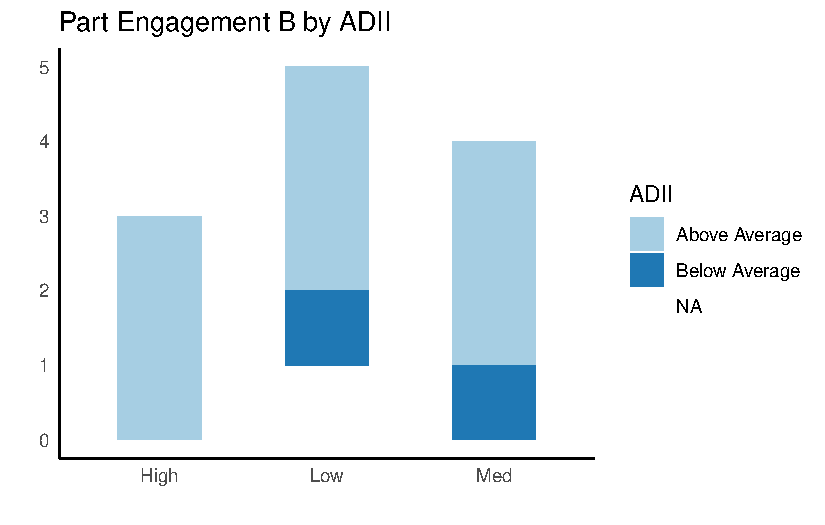
\includegraphics{report_files/figure-pdf/unnamed-chunk-19-11.pdf}

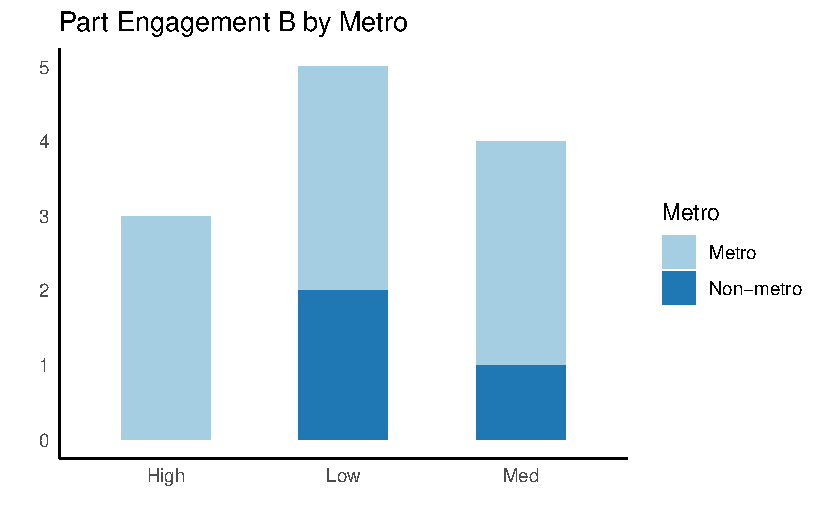
\includegraphics{report_files/figure-pdf/unnamed-chunk-19-12.pdf}

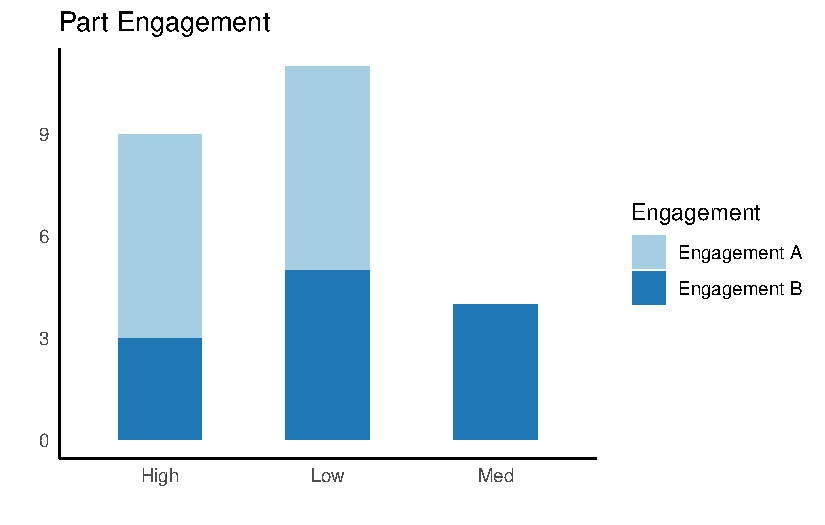
\includegraphics{report_files/figure-pdf/unnamed-chunk-19-13.pdf}

Figure 18.How well-placed schools believe they are to prevent a
situation: pre- vs.~post-Part B: self-assessment

Pre-post 1

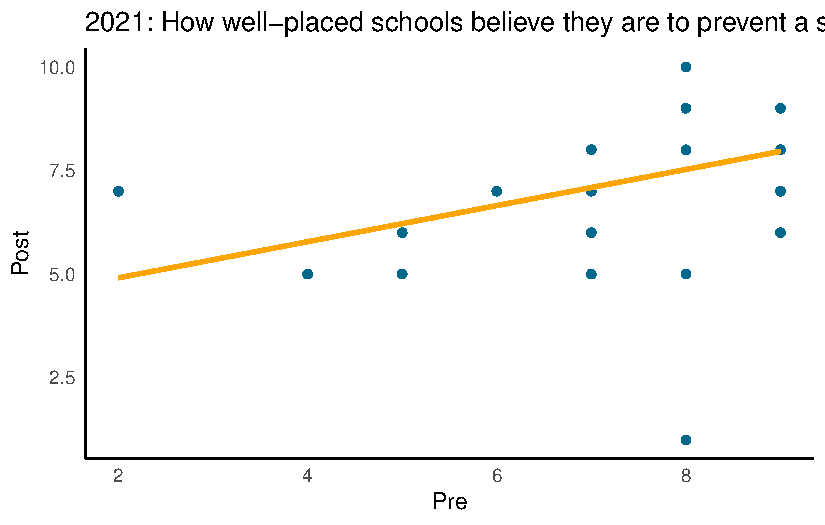
\includegraphics{report_files/figure-pdf/unnamed-chunk-20-1.pdf}

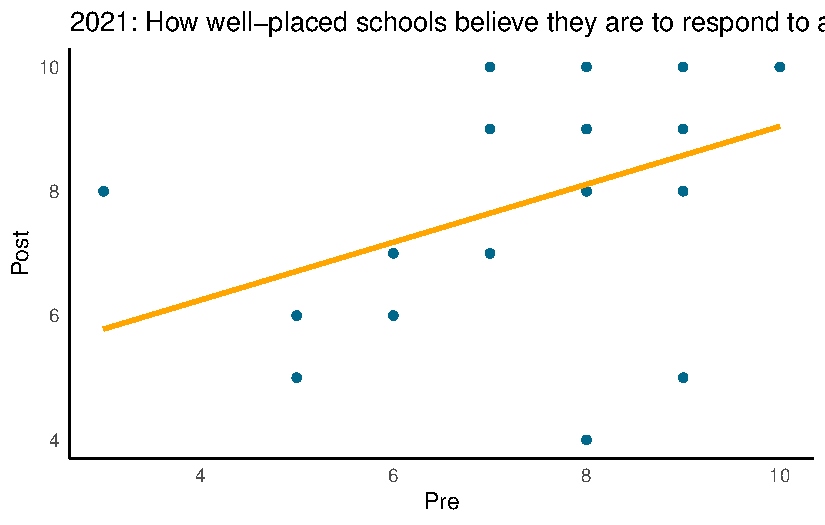
\includegraphics{report_files/figure-pdf/unnamed-chunk-20-2.pdf}

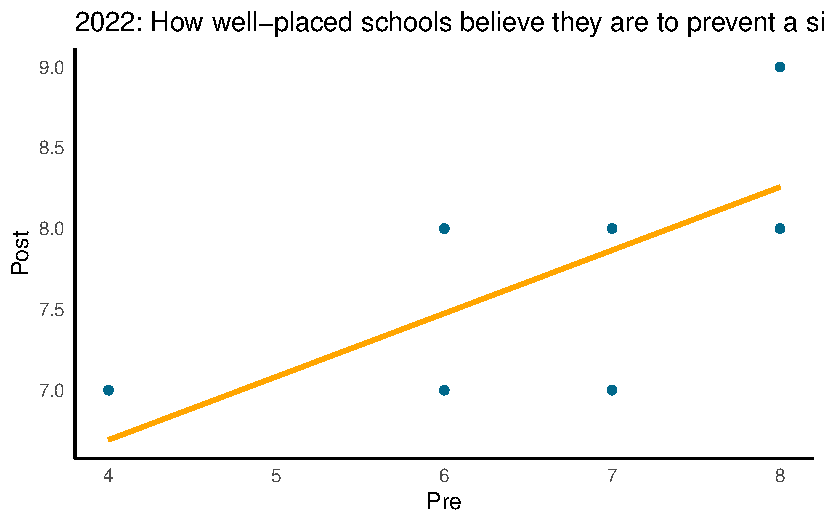
\includegraphics{report_files/figure-pdf/unnamed-chunk-20-3.pdf}

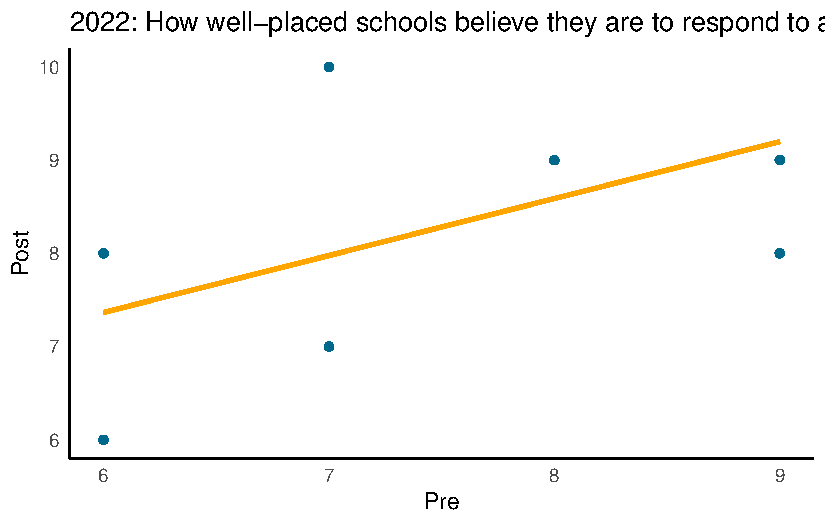
\includegraphics{report_files/figure-pdf/unnamed-chunk-20-4.pdf}

Figure 19. How well-placed schools believe they are to respond to a
situation: pre- vs.~post-Part B: self-assessment/

Figure 20. Comparison of Part A and Part B scores - all schools

Figure 21. two bar charts that include the 2021 vs.~2022 results for the
six schools that completed the instrument both years -- by Domain and
total for Part A, and by Focus Area and total for Part B. \#\# Results

{[}Repeat charts from 2021 report, but with comparison to 2022 data. So,
for example, bar charts would show both 2021 data (striped) next to 2022
data (solid). If charts get too crowded/too hard to read, can present
side-by-side or vertically. Test for any statistically significant
differences and indicate in chart.{]}

\hypertarget{part-a-results}{%
\subsubsection{Part A Results}\label{part-a-results}}

\hypertarget{part-b-results}{%
\subsubsection{Part B Results}\label{part-b-results}}

\hypertarget{summary-quantitative-results}{%
\subsection{Summary -- quantitative
results}\label{summary-quantitative-results}}

  \#\# Discussion {[}Integration of quant and qual results{]} \#\#
Conclusion \#\# References \#\# Appendices



\end{document}
